\subsubsection{Client-Server-Architekturen}
\label{sec:Kap-7.1.2.2}

Client-Server-Architekturen werden für webbasierte Softwaresysteme verwendet. Es gibt verschiedene Ausprägungen von Client-Server-Architekturen, aber das Grundprinzip ist immer dasselbe: Als Client dient der Computer bzw. das Mobilgerät des Nutzers, über den, zum Beispiel durch Browser oder App, mit der Benutzungs\-oberfläche interagiert werden kann. Die Softwareanwendung selber wird als eine Menge von Diensten organisiert, die auf einem oder mehreren entfernten Servern laufen. Die Clients der Nutzer greifen auf die benötigten Dienste zu und präsentieren dem Nutzer die Ergebnisse. Abbildung~\ref{fig:client_server_architektur} zeigt die Funktionsweise einer Client-Server-Architektur auf einer hohen Abstraktionsebene.

\vspace{\baselineskip} %%% für Druck
\vspace{\baselineskip} %%% für Druck

\begin{figure}[h!]
	\centering
	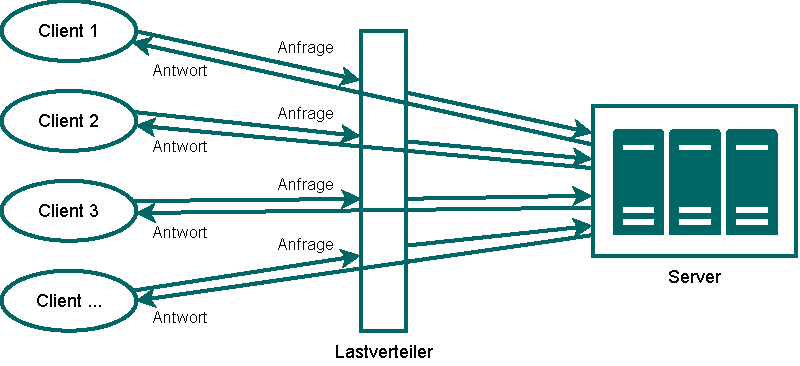
\includegraphics{Bilder/Kapitel-7/client_server_architektur.pdf}
	\caption[Client-Server-Architektur]{Client-Server-Architektur, nach \cite[114]{som20}}
	\label{fig:client_server_architektur}
\end{figure}

\vspace{\baselineskip} %%% für Druck

Auf Serverseite handelt es sich meistens nicht um einen einzigen Server, sondern um einen Serververbund, 
\marginline{Serververbund und Lastverteiler} 
an dem unterschiedlich viele Server beteiligt sein können. Client-Server-Architekturen sind darauf ausgerichtet, dass viele Clients unabhängig und ohne Kenntnis voneinander Anfragen an den Serververbund schicken können. Ein sogenannter Lastverteiler (engl. Load Balancer) verteilt die Anfragen an die beteiligten Server, um das Gesamtsystem auch bei großer Anzahl gleichzeitig eintreffender Anfragen performant zu halten. Der Lastverteiler selber ist entweder ein spezielles Hardwaregerät oder eine Load Balancing-Softwareanwendung auf einem Server. Im Unterschied zu den Servern im Serververbund ist dieser nicht an den zu erbringenden Diensten der eigentlichen Anwendungssoftware beteiligt, seine einzige Aufgabe besteht darin, die Anfragen geeignet zu verteilen.

Die Aufgabe der Clients 
\marginline{Aufgabengebiet der Clients} 
in Client-Server-Architekturen besteht mindestens darin, die Interaktion mit den Benutzern zu übernehmen. Zu Anfangszeiten von Client-Server-Architekturmodellen hatten die Clients häufig nur wenig Rechenkapazität. Ihre Tätigkeit war daher auf den Bereich der Nutzerinteraktion beschränkt, die gesamte Verarbeitung innerhalb des Softwaresystems fand auf dem Serververbund statt. Heute haben selbst Smartphones so viel Rechenkapazität, dass in vielen Software\-anwendungen die Clients neben der reinen Benutzerinteraktion auch für einen Teil der Datenverarbeitung zuständig sind. Das Prinzip der Zusammenarbeit von Client-Seite und Server-Seite ist aber nach wie vor dasselbe, nur die Arbeitsaufteilung unterscheidet sich.

\vspace{2mm} %%% für Druck

Client-Server-Architekturen und die zuvor vorgestellte Schichtenarchitektur \marginline{Bezug zur Schichten\-architektur} sind durchaus keine sich ausschließenden Architekturalternativen, sondern werden häufig in Kombination eingesetzt. Dafür wird innerhalb der Client-Server-Architektur das eigentliche Anwendungssystem nach Schichtenarchitektur organisiert. Client-Seite und Server-Seite sind dann jeweils für unterschiedliche Schichten verantwortlich. Abbildung~\ref{fig:schichtenarchitektur_fuer_client_server_architektur} zeigt eine Schichtenarchitektur, wie sie innerhalb von Client-Server-Ar\-chi\-tek\-tu\-ren vorkommen kann. Die Client-Seite ist für die Funktionalitäten der Präsentationsschicht zuständig, die Server-Seite für die drei anderen Schichten (sogenanntes Thin-Client-Modell). Die Client-Seite kann, wie im vorherigen Absatz beschrieben, aber auch zusätzlich für die Schicht Anwendungsverarbeitung zuständig sein, dann bleiben auf Server-Seite nur die beiden Schichten Datenbank und Datenverwaltung (Fat-Client-Modell). Man nennt diese Art der Architektur „zweischichtige Client-Server-Architektur“, wobei sich die „zwei“ auf die beiden Schichten Client und Server bezieht und nicht auf die Anzahl der Schichten der Anwendungssoftware.

\vspace{\baselineskip} %%% für Druck

\begin{figure}[h!]
	\centering
	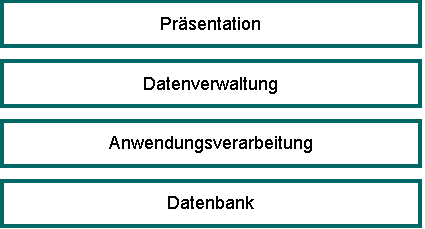
\includegraphics{Bilder/Kapitel-7/schichtenarchitektur_fuer_client_server_architektur.pdf}
	\vspace{2mm} %%% für Druck
	\caption[Schichtenarchitektur für eine Client-Server-Architektur]{Schichtenarchitektur für eine Client-Server-Architektur, nach \cite[564]{som18}}
	\label{fig:schichtenarchitektur_fuer_client_server_architektur}
\end{figure}

\vspace{\baselineskip} %%% für Druck

Alternativ zu den zweischichtigen Architekturen gibt es die mehrschichtigen Client-Server-Architekturen. Im Unterschied zu den zweischichtigen Architekturen wird hier die Serverseite noch weiter unterteilt. Abbildung~\ref{fig:client_server_architektur_mehrschichtig} zeigt eine heute übliche mehrschichtige Client-Server-Architektur mit Unterteilung in einen Webserver, einen Anwendungsserver und einen Datenbankserver. Alle drei Serverarten können natürlich auch mehrfach im Serververbund vorkommen, und zusätzlich können für die Skalierbarkeit der Anwendung wieder Lastverteilungsmechanismen vorhanden sein. Sehr ausführliche Informationen zu den hier beschriebenen und weiteren Client-Server-Architekturen finden Sie bei \cite[562-581]{som18}.

\begin{figure}[h!]
	\centering
	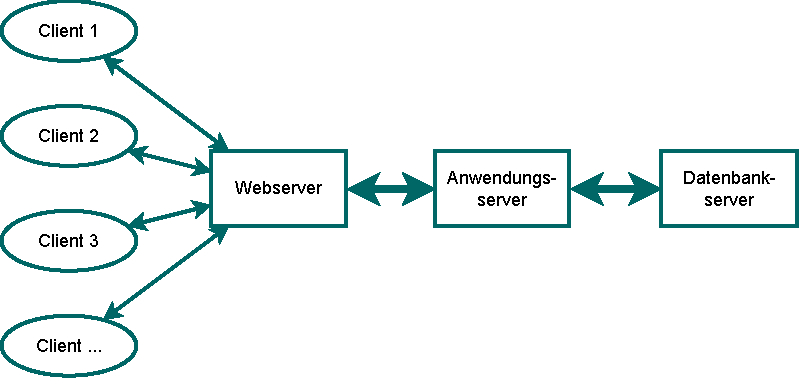
\includegraphics{Bilder/Kapitel-7/client_server_architektur_mehrschichtig.pdf}
	\caption[Mehrschichtige Client-Server-Architektur]{Mehrschichtige Client-Server-Architektur, nach \cite[117]{som20}}
	\label{fig:client_server_architektur_mehrschichtig}
\end{figure}

% Möglichkeit hier noch SOA zu thematisieren

\minisec{MVC-Muster}
\vspace{1mm} %%% für Druck

Innerhalb des Bereichs der Client-Server-Architekturmuster spielt ein weiteres 
\linebreak %%% für Druck
Muster eine wichtige Rolle, das sogenannte MVC-Muster.

MVC steht für Model-View-Controller. Zielsetzung des Musters ist die Entkopplung zwischen dem Modell (Daten und Geschäftslogik) einer Soft\-ware\-an\-wen\-dung und der Darstellung der Ausgabe. Dafür werden drei Komponenten Modell, Sicht und Programmsteuerung voneinander unabhängig gehalten und die notwendige Kommunikation zwischen ihnen findet nur über einen festgelegten Mechanismus statt. Das MVC-Muster wird sowohl als Architekturmuster – und dort nicht nur im Rahmen von Client-Server-Architekturen – als auch als Entwurfsmuster eingesetzt. Entwurfs\-muster operieren auf der Ebene der Klassen und Objekte, also auf einer deutlich niedrigeren Abstraktionsebene als Architekturmuster. Im Rahmen von Client-Server-Architekturen wird das MVC-Muster für die Organisation der Interaktion zwischen Client und Server verwendet. 

Es gibt das MVC-Muster aufgrund seiner verschiedenen Einsatzbereiche in verschiedenen Varianten. Etwas grundlegendere Unterschiede zwischen den Varianten bestehen einerseits in der Kommunikationsgestaltung zwischen Model und View und andererseits (bei Verwendung in Client-Server-Architekturen) in der Aufteilung der Komponentenzuständigkeit auf Client und Server. Die wesentliche Verfahrensweise des Musters ist aber gleich: Durch die Trennung von Model und View kann es mehrere Views zu einem Modell geben, die Daten des Modells damit in unterschiedlicher Weise dargestellt werden. Abbildung~\ref{fig:mvc_muster} zeigt eine Variante des MVC-Musters. 

\begin{figure}[h!]
	\centering
	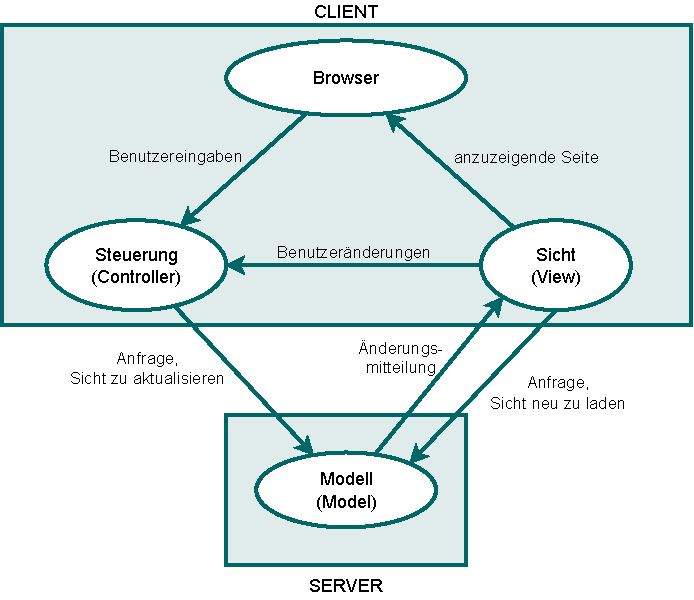
\includegraphics{Bilder/Kapitel-7/mvc_muster.pdf}
	\caption[Das MVC-Muster im Rahmen einer Client-Server-Architektur]{Das MVC-Muster im Rahmen einer Client-Server-Architektur, nach \cite[115]{som20}}
	\label{fig:mvc_muster}
\end{figure}

Auf jedem Client kann es mehrere Views geben, in denen die Daten unterschiedlich dargestellt sind. Die Views sind dabei unabhängig voneinander und zwar sowohl bezogen auf diesen einen Client als auch in Bezug zu den Views der anderen Clients. Jede View registriert sich bei dem Model. Das Model benachrichtigt alle bei ihm registrierten Clients, wenn sich Daten geändert haben, so dass die Views sich aktualisieren können. Benutzereingaben, die etwas am Modell ändern würden, werden über die Controller-Komponente des Musters behandelt.
